\documentclass[12pt,letterpaper]{article}
\usepackage{amsmath}
\usepackage{gensymb}
\usepackage{enumitem}
\usepackage{graphicx}
\usepackage[margin=1in]{geometry}
\setlength{\parindent}{0pt}
\title{Physics Club Practice Test 1}
\usepackage[export]{adjustbox}
\usepackage[none]{hyphenat}
\usepackage{titlesec}
\titlespacing{\section}{0pt}{4.0ex plus .2ex}{-3.3ex}
\titlespacing{\paragraph}{0pt}{0pt}{1em}
% \setenumerate[2]{label={\alph*.}}
\usepackage{fancyhdr}
\fancypagestyle{firstpage}
{
	\renewcommand{\headrulewidth}{0pt}
	\renewcommand{\footrulewidth}{0.4pt}
	\lfoot{Physics Club}
	\cfoot{$F=ma$ Practice Test 1}
	\rfoot{\thepage}
}
\thispagestyle{firstpage}
\pagestyle{fancy}
\fancyhf{}
\renewcommand{\headrulewidth}{0pt}
\renewcommand{\footrulewidth}{0.4pt}
\lfoot{Physics Club}
\cfoot{$F=ma$ Practice Test 1}
\rfoot{\thepage}
\begin{document}
\section*{Physics Club: $F=ma$ Practice Test 1}\hfill Version 1.1
\vspace{-2.5pt}
\begin{center}
\textsc{25 Questions -- 75 Minutes}
\end{center}
\vspace{-5pt}
Assume the acceleration due to gravity near the surface of the Earth $g = 10$ m/s$^2$.
\smallskip

Correct answers will be awarded one point; incorrect answers will result in a deduction of 1/4 point. There is no penalty for leaving an answer blank.
\smallskip

You may use a scientific calculator. Its memory must be cleared of data and programs.
% \vspace{-7.5pt}

\hrulefill

\begin{enumerate}

% --- F=ma Question ---
% \item
% A 0.3 kg apple falls from rest through a height of 50 cm onto a flat surface. Upon impact, the apple comes to rest in 0.2 s, and 5 cm$^2$ of the apple comes into contact with the surface during the impact. What is the average pressure exerted upon the apple during the impact?
% \begin{enumerate}
% \item 25 000 Pa
% \item 19 000 Pa
% \item 9500 Pa
% \item 95 Pa
% \item 4.7 Pa
% \end{enumerate}
% \end{enumerate}

% --- F=ma Question ---
% \textbf{The following information is used for questions 2 and 3.}\\
% Three blocks of identical mass are placed on a frictionless table as shown. The center block is at rest, whereas the other two blocks are moving directly toward it at identical speeds $v$. The center block is initially closer to the left block than the right one. All motion takes place along a single horizontal line.

% --- F=ma Question ---
% \begin{enumerate}[resume]
% \item
% Suppose that all collisions are instantaneous and perfectly elastic. After a long time, which of the following is true?
% \begin{enumerate}
% \item The center block is at rest somewhere to the left of its initial position.
% \item The center block is at rest at its initial position.
% \item The center block is moving to the left.
% \item The center block is at rest somewhere to the right of its initial position.
% \item The center block is moving to the right.
% \end{enumerate}

% --- F=ma Question ---
% \item
% Suppose, instead, that all collisions are instantaneous and perfectly inelastic. After a long time, which of the following is true?
% \begin{enumerate}
% \item The center block is at rest somewhere to the left of its initial position.
% \item The center block is at rest at its initial position.
% \item The center block is moving to the left.
% \item The center block is at rest somewhere to the right of its initial position.
% \item The center block is moving to the right.
% \end{enumerate}

% --- F=ma Question ---
% \item
% A spaceman of mass 80 kg is sitting in a spacecraft near the surface of the Earth. The spacecraft is accelerating downward at one-third of the acceleration due to gravity. What is the force on the spacecraft by the spaceman?
% \begin{enumerate}
% \item 4800 N
% \item 4000 N
% \item 3200 N
% \item 800 N
% \item 530 N
% \end{enumerate}

\item
Starting from rest at time $t = 0$, a car moves in a straight line with an acceleration given by the accompanying graph. What is the speed of the car at $t = 2$ s?

\begin{tabular}{l r}

\begin{minipage}{0.575\textwidth}
\begin{enumerate}
\item 1.0 m/s
\item 2.0 m/s
\item 8.0 m/s
\item 10.5 m/s
\item 12.5 m/s
\end{enumerate}
\end{minipage} &
\begin{minipage}{0.4\textwidth}
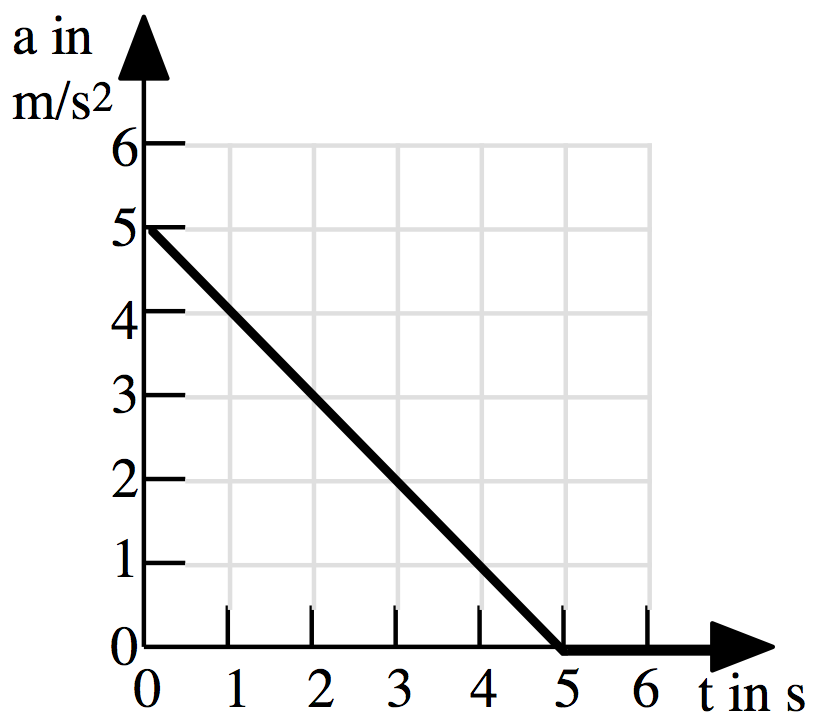
\includegraphics[width=0.65\textwidth,center]{agraph.png}
\end{minipage}
\end{tabular}
\end{enumerate}

\textbf{The following information is used for questions 2 and 3.}\\
A flare is dropped from a plane flying over level ground at a velocity of 70 m/s in the horizontal direction. At the instant the flare is released, the plane begins to accelerate horizontally at 1.75 m/s$^2$. The flare takes 4.5 s to reach the ground.

\begin{enumerate}[resume]
\item
Relative to a spot directly under the flare at release, the flare lands
\begin{enumerate}
\item directly on the spot.
\item 333 m in front of the spot.
\item 274 m in front of the spot.
\item 280 m in front of the spot.
\item 315 m in front of the spot.
\end{enumerate}

\item
As seen by the pilot of the plane and measured relative to a spot directly under the plane when the flare lands, the flare lands
\begin{enumerate}
\item 333 m behind the plane.
\item 18 m behind the plane.
\item directly under the plane.
\item 36 m in front of the plane.
\item 315 m in front of the plane.
\end{enumerate}

\vfill
\newpage

\item
A certain football quarterback can throw a football a maximum range of 76 meters on level ground. What is the highest point reached by the football when this maximum range is thrown?
\begin{enumerate}
\item 76 m
\item 54 m
\item 38 m
\item 28 m
\item 19 m
\end{enumerate}

\item
A car of mass $m$ is slipping down a slope of inclination angle $\theta$ at a constant acceleration $a$. The coefficient of static friction between the wheels and the slope is $\mu$. What is the frictional force between the wheels and the slope?
\begin{enumerate}
\item $\mu mg\cos\theta$
\item $\mu mg$
\item $mg\left(\sin\theta-\mu\right)$
\item $m\left(g-a\right)$
\item $mg\sin\theta-ma$
\end{enumerate}

\item
Which solid vector in the accompanying figures best represents the acceleration of the pendulum mass at the intermediate point in its swing indicated?

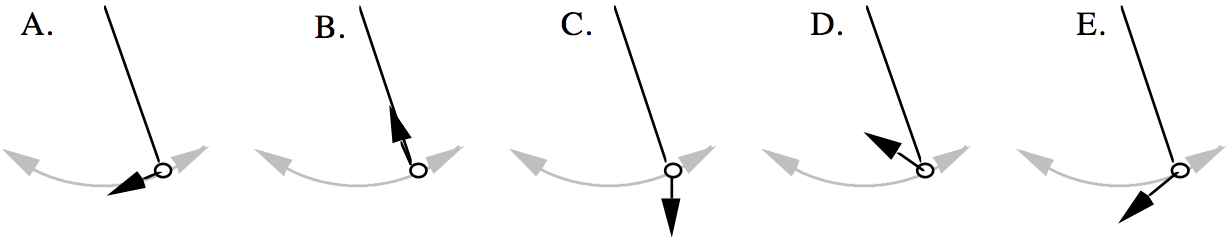
\includegraphics[width=0.9\textwidth,center]{swing.png}

% \item
% A force $F$ is used to hold two blocks of mass $m_1$ and $m_2$ on an incline as shown in the diagram. The plane makes an angle $\theta$ with the horizontal and $F$ is perpendicular to the plane. The coefficients of static friction between the plane and the block $m_2$ and between the two blocks are both equal to $\mu$ with $\mu < \tan\theta$. What is the minimum force $F$ necessary to keep both blocks at rest?
% \begin{enumerate}
% \item $\mu\left(m_1+m_2\right)$
% \item $\left(m_1+m_2\right)g\cos\theta$
% \item $\displaystyle m_1g\left(\frac{\sin\theta}{\mu}-\cos\theta\right)$
% \item $\displaystyle m_2g\left(\frac{\sin\theta}{\mu}-\cos\theta\right)$
% \item $\displaystyle \left(m_1+m_2\right)g\left(\frac{\sin\theta}{\mu}-\cos\theta\right)$
% \end{enumerate}

\item
A ball of mass $m$ is fastened to a string. The ball swings in a vertical circle of radius $R$ with the other end of the string held fixed. The difference between the string's tension at the bottom of the circle and at the top is
\begin{enumerate}
\item $8mg$.
\item $6mg$.
\item $4mg$.
\item $2mg$.
\item $mg$.
\end{enumerate}

% --- F=ma Question ---
% \item
% You are given a standard kilogram mass and a tuning fork that is calibrated in Hz. You are also provided with a complete collection of laboratory equipment, but none of it is calibrated in SI units. You do not know the values of any fundamental constants. Which of the following quantities could you measure in SI units?
% \begin{enumerate}
% \item The density of a block of ice
% \item The acceleration due to gravity
% \item The spring constant of a given spring
% \item The speed of sound in the air
% \item The air temperature in the room
% \end{enumerate}

% --- F=ma Question ---
% \item
% Satellite A of mass $2m$, B of mass $3m$, and C of mass $4m$ are in coplanar orbits around a planet as shown in the figure. Satellite A is in a circular orbit of radius $2R$ and C is in a circular orbit of radius $R$. Satellite B is in an elliptical orbit. The minimum distance between satellite B and the planet is $R$. The maximum distance between the satellite B and the planet is $2R$. The magnitudes of the angular momenta of the satellites as measured about the plant are $L_A$, $L_B$, and $L_C$. Which of the following statements is correct?
% \begin{enumerate}
% \item $L_C > L_A > L_B$
% \item $L_C > L_B > L_A$
% \item $L_B > L_C > L_A$
% \item $L_B > L_A > L_C$
% \item The relationship between the magnitudes is different at various instants in time.
% \end{enumerate}
% \end{enumerate}

% --- F=ma Question ---
% \textbf{The following information is used for questions 15 and 16.}\\
% Two stars orbit their common center of mass as shown in the diagram below. The masses of the two stars are $9M$ and $M$. The distance between the stars is $d$.

% --- F=ma Question ---
% \begin{enumerate}[resume]
% \item
% What is the value of the gravitational potential energy of the two star system?
% \begin{enumerate}
% \item $-GM^2$/$d$
% \item $-9GM^2$/$d$
% \item $-GM^2$/$d^2$
% \item $9GM^2$/$d$
% \item $-9GM^2$/$d^2$
% \end{enumerate}

% --- F=ma Question ---
% \item Determine the period of orbit for the star of mass $9M$.
% \begin{enumerate}
% \item $\displaystyle \pi\sqrt\frac{2d^3}{5GM}$
% \item $\displaystyle \frac{2\pi}{5}\sqrt\frac{d^3}{GM}$
% \item $\displaystyle \pi\sqrt\frac{2d^2}{5GM}$
% \item $\displaystyle \frac{2\pi}{3}\sqrt\frac{d^3}{GM}$
% \item $\displaystyle \pi\sqrt\frac{2d^3}{3GM}$
% \end{enumerate}

% \item
% As shown, a big box of mass $M$ is resting on a horizontal smooth floor. On the bottom of the box there is a small box also of mass $M$. The block is given an initial peed $v_0$ relative to the floor, and starts to bounce back and forth between the two walls of the box. Find the final speed of the box when the block has finally come to rest in the box.
% \begin{enumerate}
% \item 0
% \item $v_0$
% \item $v_0$/2
% \item $v_0$/3
% \item $v_0$/4
% \end{enumerate}

\vfill
\newpage

\item
Two objects of mass $m$ and $3m$ are placed at either end of a spring of spring constant $k$ and the whole system is placed on a horizontal frictionless surface. At what angular frequency $\omega$ does the system oscillate?
\begin{enumerate}
\item $\displaystyle \sqrt\frac{k}{m}$
\item $\displaystyle \sqrt\frac{3k}{m}$
\item $\displaystyle \sqrt\frac{3k}{2m}$
\item $\displaystyle \sqrt\frac{2k}{3m}$
\item $\displaystyle \sqrt\frac{4k}{3m}$
\end{enumerate}

% \item
% Two astronauts, A and B, both with mass of 60 kg, are moving along a straight line in the same direction in a ``weightless'' spaceship. Relative to the spaceship the speed of A is 2 m/s and that of B is 1 m/s. A is carrying a bag of mass 8 kg with him. To avoid collision with B, A throws the bag with a speed $v$ relative to the spaceship toward B and B catches it. Find the minimum value of $v$.
% \begin{enumerate}
% \item 7.8 m/s
% \item 26.0 m/s
% \item 14.0 m/s
% \item 9.2 m/s
% \item 5.5 m/s
% \end{enumerate}

% --- F=ma Question ---
% \item
% A mass is attached to an ideal spring. At time $t=0$ the mass is released from rest from a position a distance $x_0$ from the position where the spring is at its natural length; the period of the ensuing (one-dimensional) simple harmonic motion is $T$. At what time is the power delivered to the mass by the spring first a maximum?
% \begin{enumerate}
% \item $t=0$
% \item $t=T$/8
% \item $t=T$/4
% \item $t=3T$/8
% \item $t=T$/2
% \end{enumerate}

\item
Two uniform circular disks of the same material and thickness are adhered together at point N. Both disks lie in the same vertical plane. The rigid body is hinged at point P and it can rotate freely about P in the vertical plane.  PO $\perp$ OM and ON $= 3$ NM, where point O and point M are the centers of the disks. When static equilibrium is reached, find the angle $\theta$ between PO and the vertical direction.

\begin{tabular}{l r}

\begin{minipage}{0.6\textwidth}
\begin{enumerate}
\item $16.7\degree$
\item $26.6\degree$
\item $30\degree$
\item $5.2\degree$
\item $7.6\degree$
\end{enumerate}
\end{minipage} &
\begin{minipage}{0.3\textwidth}
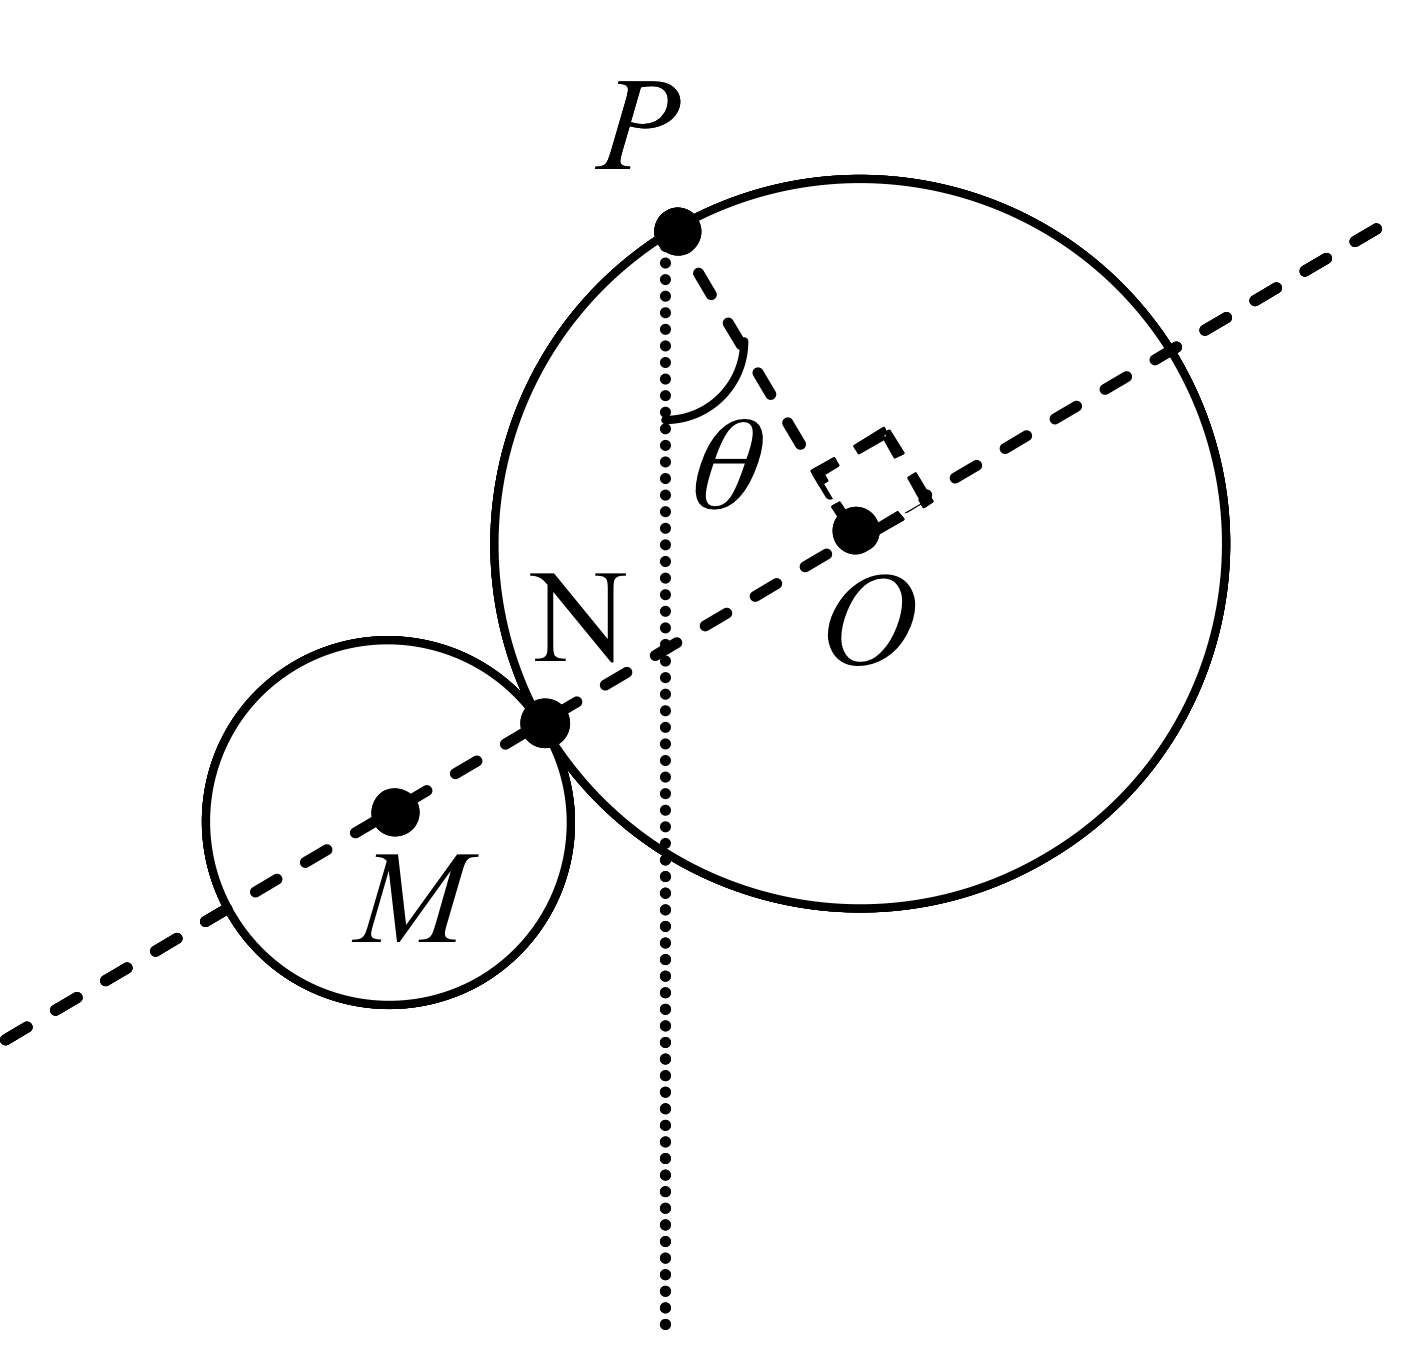
\includegraphics[width=\textwidth,left]{disks.png}
\end{minipage}
\end{tabular}

% \item
% A uniform rectangular wood block of mass $M$, with length $a$ and height $b=3a$, rests on an incline as shown. The incline and the wood block have a coefficient of static friction $\mu_s$. The incline is moved upward from an angle of zero through and angle $\theta$. At some critical angle the block will either tip over or the block will tip over (and not slip) at the critical angle.
% \begin{enumerate}
% \item $\mu_s > 1$/3
% \item $\mu_s > 2$/2
% \item $\mu_s > 1$/2
% \item $\mu_s < 1$/3
% \item $\mu_s < 2$/3
% \end{enumerate}

% --- F=ma Question ---
% \item
% Two disks are mounted on thin, lightweight rods oriented through their centers and normal to the disks. These axles are constrained to be vertical at all times, and the disks can pivot frictionlessly on the rods. The disks have identical thickness and are made of the same material, but have differing radii $r_1$ and $r_2$ with $r_1=3r_2$. The disks are given angular velocities of magnitudes $\omega_1$ and $\omega_2$, respectively, and brought into contact at their edges. After the disks interact via friction it is found that both disks come exactly to a halt. Which of the following must hold? Ignore effects associated with the vertical rods.
% \begin{enumerate}
% \item $27\omega_1 = \omega_2$
% \item $\omega_1 = 27\omega_2$
% \item $3\omega_1 = \omega_2$
% \item $\omega_1 = 3\omega_2$
% \item $9\omega_1 = \omega_2$
% \end{enumerate}
% \end{enumerate}

% --- F=ma Question ---
% \textbf{The following information is used for questions 24 and 25.}\\
% A massless elastic cord (that obeys Hooke's Law) will break if the tension in the cord exceeds a maximum value $T_\text{max}$. One end of the cord is attached to a fixed point, the other is attached to an object of mass $2m$. If a second, smaller object of mass $m$ moving at an initial speed $v_0$ strikes the larger mass and the two stick together, the cord will stretch and break, but the final kinetic energy of the two masses will be zero. If instead the two collide with a perfectly elastic one-dimensional collision, the cord will still break, and the larger mass wil move off with a final speed of $v_f$ All motion occurs on a horizontal, frictionless surface.

% --- F=ma Question ---
% \begin{enumerate}[resume]
% \item What is $v_f$/$v_0$?
% \begin{enumerate}
% \item 1/$\sqrt{2}$
% \item $\sqrt{11}$/10
% \item $\sqrt{10}$/6
% \item 1/$\sqrt{3}$
% \item $\sqrt{5/18}$
% \end{enumerate}

% --- F=ma Question ---
% \item
% Find the ratio of the total kinetic energy of the system of two masses after the perfectly elastic collision and the cord has broken to the initial kinetic energy of the smaller mass prior to the collision.
% \begin{enumerate}
% \item 1/4
% \item 2/3
% \item 1/2
% \item 3/4
% \item 4/5
% \end{enumerate}

% --- F=ma Question ---
% \item
% A person standing on the edge of a fire escape simultaneously launches two apples, one straight up with a speed of 6 m/s and the other straight down at the same speed. How far apart are the two apples 2.5 seconds after they were thrown, assuming that neither has hit the ground?
% \begin{enumerate}
% \item 14 m
% \item 21 m
% \item 30 m
% \item 41 m
% \item 54 m
% \end{enumerate}

% \item
% A car is moving with constant speed $v=10$ m/s along a straight line. A ball is thrown out at a height of 15 m with initial speed $\sqrt{2}v$ when the car is just passing below. The angle above the horizontal at which the ball is thrown is such that the ball will hit the car. Find the horizontal distance the car travels from the time the ball is thrown to the time the car is hit.
% \begin{enumerate}
% \item 45 m
% \item 40 m
% \item 35 m
% \item 30 m
% \item 25 m
% \end{enumerate}

% --- F=ma Question ---
% \item
% A 2.0 kg mass undergoes an acceleration as shown below. How much work is done on the mass?
% \begin{enumerate}
% \item $-32$ J
% \item $-16$ J
% \item 5 J
% \item 16 J
% \item 32 J
% \end{enumerate}

% \item
% As shown in the diagram, a man pushes forward on the compartment which is accelerating uniformly to the left relative to the ground. The man stays at rest relative to the compartment. Which of the following statements in respect to the ground reference frame is correct?
% \begin{enumerate}
% \item The man does positive work on the compartment.
% \item The man does negative work on the compartment.
% \item The man does zero work on the compartment.
% \item It cannot be determined
% \item Both (a) and (c) can be correct.
% \end{enumerate}

% --- F=ma Question ---
% \item
% A wooden block of mass $M$ is hung from a peg by a massless rope. A speeding bullet of mass $m$ and initial speed $v_0$ collides with the block at time $t=0$ and embeds in it. Let S be the system consisting of the block and bullet. Which quantities are conserved between $t=-8$ s and $t=+8$ s?
% \begin{enumerate}
% \item The total linear momentum of S.
% \item The horizontal component of the linear momentum of S.
% \item The mechanical energy of S.
% \item The angular momentum of S as measured about a perpendicular axis through the peg.
% \item None of the above are conserved.
% \end{enumerate}

% --- F=ma Question ---
% \item
% Lucy (mass 33.1 kg), Mary (mass 61.7 kg), and Henry (mass 24.3 kg) sit on a lightweight seesaw at evenly spaced 2.79 m intervals (in the order in which they are listed; Mary is between Lucy and Henry) so that the seesaw balances. Who exerts the most torque (in terms of magnitude) on the seesaw about the pivot point of the seesaw?
% \begin{enumerate}
% \item Henry
% \item Lucy
% \item Mary
% \item They all exert the same torque.
% \item There is not enough information to answer the question.
% \end{enumerate}

\item
A uniform 2 kg cylinder rests on a laboratory trolley as shown. The coefficient of static friction between the cylinder and the trolley is 0.5. If the cylinder is 4 cm in diameter and 10 cm in height, what is the condition on the acceleration $a$ of the trolley to cause the cylinder to tip over?

\begin{tabular}{l r}

\begin{minipage}{0.6\textwidth}
\begin{enumerate}
\item $a > 2.5$ m/s$^2$
\item $a < 2.5$ m/s$^2$
\item $a > 5$ m/s$^2$
\item $a > 4$ m/s$^2$
\item The cylinder would tip over at any acceleration.
\end{enumerate}
\end{minipage} &
\begin{minipage}{0.4\textwidth}
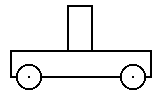
\includegraphics[width=0.65\textwidth,center]{trolley.png}
\end{minipage}
\end{tabular}

% --- F=ma Question ---
% \item A flat uniform disk of mass 40 kg and radius 1 m rotates about an axis perpendicular to the plane of the disk and through the center of the disk. A net constant resistive torque acting on the disk between 0 and 3 seconds causes the angular velocity of the disk to vary as shown in the graph below. Find the average power dissipated due to the net resistive torque for the 3 seconds duration.
% \begin{enumerate}
% \item 50 W
% \item 40 W
% \item 30 W
% \item 20 W
% \item 10 W
% \end{enumerate}

\vfill
\newpage

\item
Four masses $M$ are arranged at the vertices of a square of side length $a$. What is the gravitational potential energy of this arrangement?
\begin{enumerate}
\item $\displaystyle -\left(4+\sqrt{2}\right)\frac{GM^2}{a}$
\item $\displaystyle -\left(4-\sqrt{2}\right)\frac{GM^2}{a}$
\item $\displaystyle -4\frac{GM^2}{a}$
\item $\displaystyle -\left(2+\sqrt{2}\right)\frac{GM^2}{a}$
\item $\displaystyle -\left(2-\sqrt{2}\right)\frac{GM^2}{a}$
\end{enumerate}

\item
A particle of mass $m$ moving along the $x$-axis with speed $v$ collides with a particles of mass $2m$ initially at rest. After the collision, the first particle has come to rest, and the second particle has split into two equal-mass pieces that move at equal angle $\theta$ with the $x$-axis, as shown in the figure. Which of the following statements correctly describes the speeds of the two pieces?

\begin{tabular}{l r}

\begin{minipage}{0.5\textwidth}
\begin{enumerate}
\item Both pieces move with speed $v$.
\item One of the pieces moves with speed $v$, the other moves with speed less than $v$.
\item Both pieces move with speed $v$/2.
\item One of the pieces moves with speed $v$/2, the other moves with speed greater than $v$/2.
\item Both pieces move with speed greater than $v$/2.
\end{enumerate}
\end{minipage} &
\begin{minipage}{0.5\textwidth}
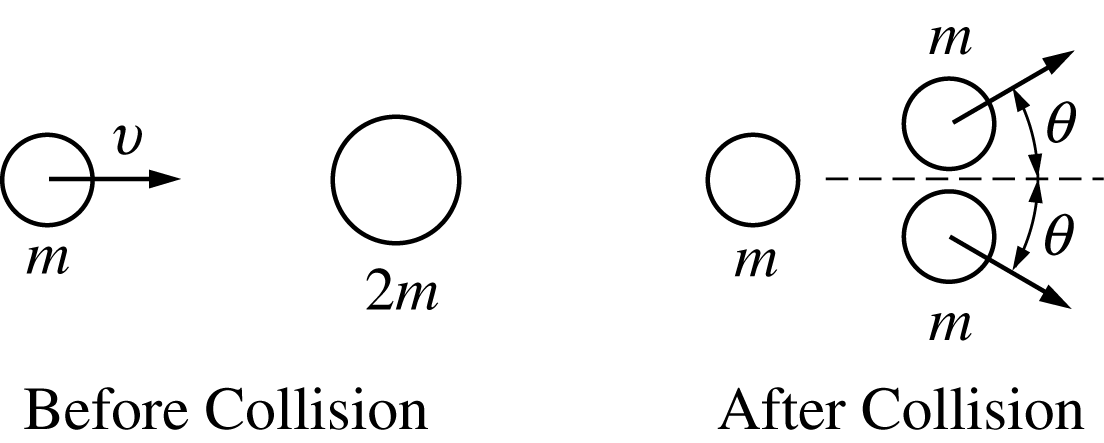
\includegraphics[width=0.75\textwidth,left]{collision.png}
\end{minipage}
\end{tabular}

\item
A spacecraft is orbiting on the surface of an unknown planet. In order to determine the density of the planet, which one of the following should be measured?
\begin{enumerate}
\item Radius of the planet
\item The volume of the planet
\item The moving speed of the spacecraft
\item The period of the motion
\item None of the above measurements would determine the density of the planet.
\end{enumerate}
\end{enumerate}

\vfill
\newpage

\textbf{The following information is used for questions 14 and 15.}\\
Two weights, both of mass $m$, are joined by a weightless spring of natural length $L$ and force constant $k$. They are placed on a smooth surface and at rest. One weight is given an impulse and acquires an initial velocity $v$ toward the other weight.

\begin{enumerate}[resume]
\item
What is the speed of the center of mass of the weights-spring system?
\begin{enumerate}
\item $0.5v$
\item $\displaystyle 0.5v - \sqrt\frac{kL^2}{2m}$
\item $\displaystyle \sqrt\frac{kL^2}{2m} - 0.5v$
\item $v$
\item $0.5v - \sqrt\frac{kL^2}{m}$
\end{enumerate}

\item
What is the minimum distance between the two weights?
\begin{enumerate}
\item $\displaystyle L - \frac{v}{2}\sqrt\frac{m}{k}$
\item $\displaystyle L - v\sqrt\frac{m}{2k}$
\item $\displaystyle L - v\sqrt\frac{m}{k}$
\item $\displaystyle v\sqrt\frac{m}{k}$
\item $\displaystyle \frac{v}{2}\sqrt\frac{m}{k}$
\end{enumerate}

\item
A rod of mass $M$ and length $L$ mass moment of inertia $\left(1/12\right)ML^2$ about its center of mass. A sphere of mass $m$ and radius $R$ has a moment of inertia $\left(2/5\right)mR^2$ about its center of mass. A combined system is formed by centering the sphere at one end of the rod and placing an axis at the other. What is the moment of inertia $I$ of the combined system about the axis shown?

\begin{tabular}{l r}

\begin{minipage}{0.4\textwidth}
\begin{enumerate}
\item $\displaystyle \frac{1}{12}ML^2 + \frac{2}{5}mR^2$
\item $\displaystyle \frac{1}{12}ML^2 + \frac{2}{5}mR^2 + ML^2$
\item $\displaystyle \frac{1}{3}ML^2 + \frac{2}{5}mR^2 + mL^2$
\item $\displaystyle \frac{1}{12}ML^2 + mL^2$
\item $\displaystyle \frac{1}{3}ML^2 + mL^2$
\end{enumerate}
\end{minipage} &
\begin{minipage}{0.5\textwidth}
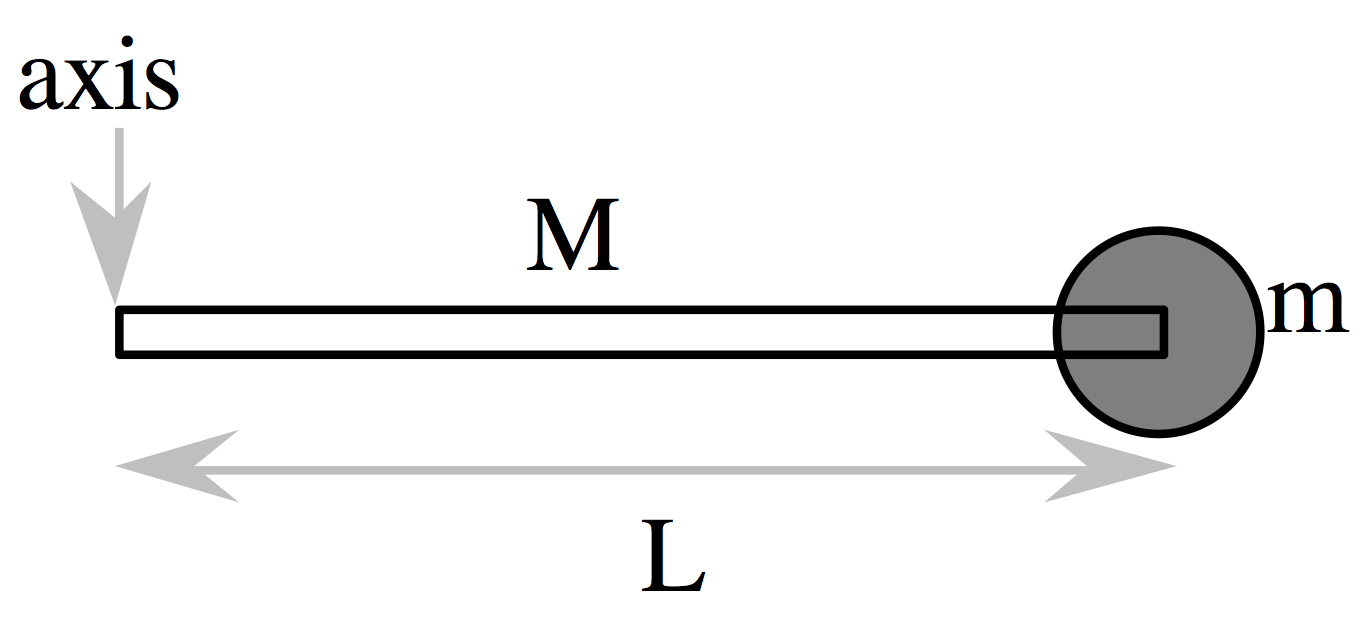
\includegraphics[width=\textwidth,left]{rod.png}
\end{minipage}
\end{tabular}

\item
The mass in the figure below slides on a frictionless surface. When the mass is pulled out, spring 1 is stretched to a distance $x_1$ from its equilibrium position and spring 2 is stretched a distance $x_2$. The spring constants are $k_1$ and $k_2$, respectively. Find the force pulling back on the mass.

\begin{tabular}{l r}

\begin{minipage}{0.35\textwidth}
\begin{enumerate}
\item $-k_2x_1$
\item $-k_1x_2$
\item $-\left(k_1x_1+k_2x_2\right)$
\item $\displaystyle -\frac{k_1+k_2}{2}\left(x_1+x_2\right)$
\item $\displaystyle -\frac{k_1k_2}{k_1+k_2}\left(x_1+x_2\right)$
\end{enumerate}
\end{minipage} &
\begin{minipage}{0.75\textwidth}
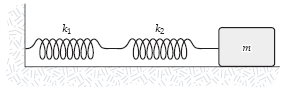
\includegraphics[width=0.75\textwidth,left]{spring.png}
\end{minipage}
\end{tabular}

\item
An object with a mass of 3 kilograms is accelerated from rest. The graph at right shows the magnitude of the net force in newtons as a function of time in seconds. At time $t=4$ seconds the object's velocity would have been closest to which of the following?

\begin{tabular}{l r}

\begin{minipage}{0.525\textwidth}
\begin{enumerate}
\item 2.3 m/s
\item 3.5 m/s
\item 5.8 m/s
\item 7.0 m/s
\item 11.5 m/s
\end{enumerate}
\end{minipage} &
\begin{minipage}{0.75\textwidth}
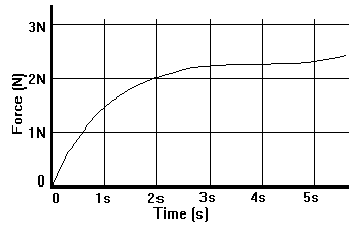
\includegraphics[width=0.5\textwidth,left]{fgraph.png}
\end{minipage}
\end{tabular}

% \item
% As shown in the figure, AB $= 3.5$ m, AC $=3.0$ m, AD $= 0.5$ m. The two rods AC and BC weight 200 N each. The floor is frictionless. Find the tension in the rope.
% \begin{enumerate}
% \item 280 N
% \item 500 N
% \item 150 N
% \item 302 N
% \item 180 N
% \end{enumerate}

\item
Three small objects, all of mass $M$, are released simultaneously from the top of three inclined planes of the same height $H$. The objects and incline angles of the corresponding incline planes are described as follows:
\begin{enumerate}[label=\Roman*.]
\item a cube of side $R$ from an incline plane with an incline angle of $30\degree$
\item a solid cylinder of radius $R$ from an incline plane with an incline angle of $45\degree$
\item a hollow cylinder of radius $R$ from an incline plane with an incline angle of $60\degree$
\end{enumerate}
Assume that the cylinders roll down their corresponding incline planes without slipping and the cube slides down the plane without friction. Which objects reach the bottom of the plane first?
\begin{enumerate}
\item I
\item II
\item III
\item I \& II
\item II \& III
\end{enumerate}

\vfill
\newpage

\item
Two monkeys of the same weight are holding tightly the two end of a rope with negligible mass. The rope passes through a smooth pulley, as shown in the figure. The two monkeys are initially at rest. Now the right monkey starts to climb up the rope at an average speed $v$ relative to the pulley to get closer to the left monkey. Let the initially vertical separation of the monkeys be $h$. Find the average velocity of the right monkey relative to the left monkey.

\begin{tabular}{l r}

\begin{minipage}{0.7\textwidth}
\begin{enumerate}
\item $2v$ upward
\item $2v$ downward
\item $v + \sqrt{2gh}$ upward
\item $v + \sqrt{2gh}$ downward
\item 0
\end{enumerate}
\end{minipage} &
\begin{minipage}{0.25\textwidth}
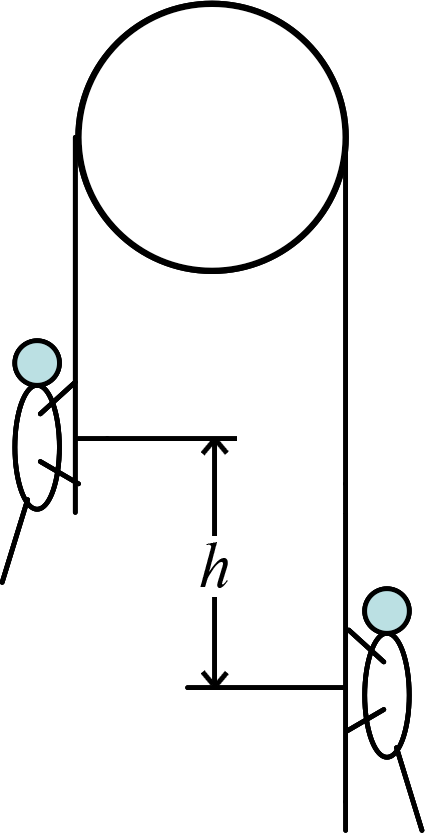
\includegraphics[width=0.75\textwidth,left]{monkey2.png}
\end{minipage}
\end{tabular}

\item
Someone is using scissors to cut a wire of circular cross section and negligible weight. The wire slides in the direction away from the hinge until the angle between the scissors blades becomes $2\alpha$. The coefficient of kinetic friction between the blades and the wire is closest to

\begin{tabular}{l r}

\begin{minipage}{0.65\textwidth}
\begin{enumerate}
\item $\sqrt{1-\tan\alpha}$.
\item $\cos{2\alpha}$.
\item $\tan{2\alpha}$.
\item $\tan\alpha$.
\item $\sqrt{2\cos^2\alpha - 1}$.
\end{enumerate}
\end{minipage} &
\begin{minipage}{0.25\textwidth}
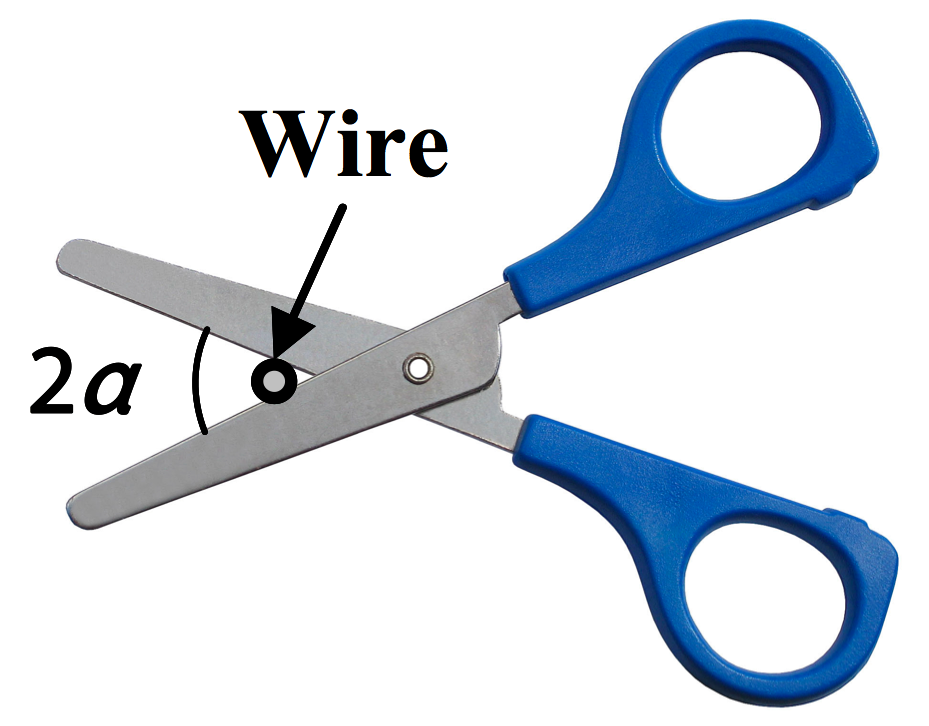
\includegraphics[width=\textwidth,left]{scissors.png}
\end{minipage}
\end{tabular}

\item
As shown in the figure, a wedge of mass $M$ is placed on a smooth inclined ramp that makes an angle $\theta$ with the horizontal. An object of mass $m$ rests on top of the wedge. The system is sliding down the ramp at acceleration $a$. Determine the apparent weight of the object $m$ as it slides down. Note that there is friction between the object and the wedge so that the object remains relatively at rest on the wedge.

\begin{tabular}{l r}

\begin{minipage}{0.6\textwidth}
\begin{enumerate}
\item $mg\cos\theta$
\item $mg\cos^2\theta$
\item $mg\sin\theta\cos\theta$
\item $mg\tan\theta$
\item $mg$
\end{enumerate}
\end{minipage} &
\begin{minipage}{0.3\textwidth}
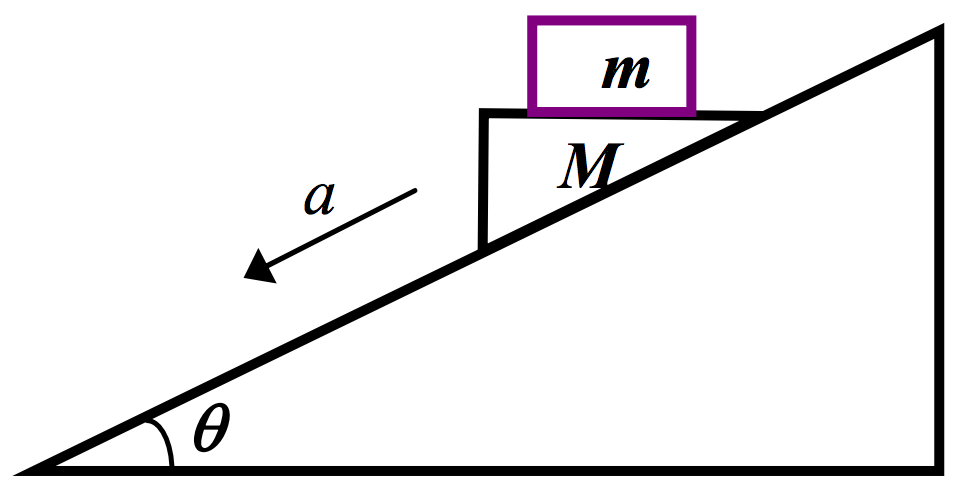
\includegraphics[width=\textwidth,left]{incline.png}
\end{minipage}
\end{tabular}

\vfill
\newpage

\item
A cup of water is placed in a car under constant acceleration to the left, as shown. Inside the water is a small air bubble. The following figures show five situations of the shape of the water surface and the direction of motion of the bubble as indicated by the arrow on the bubble. Which one is correct?

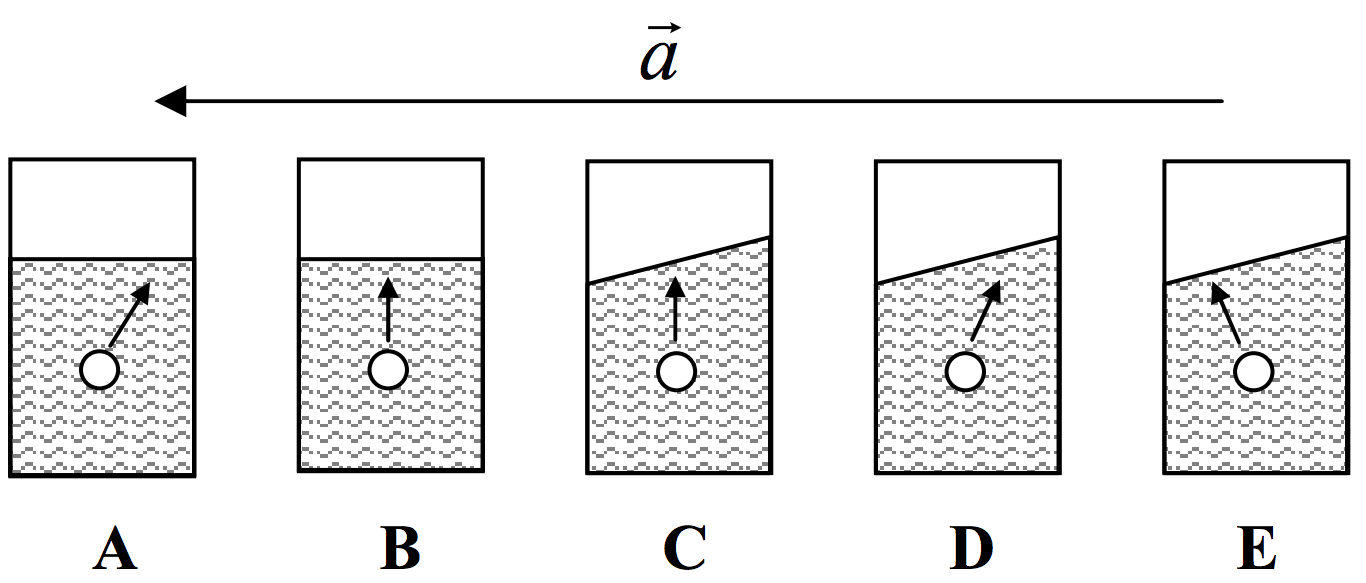
\includegraphics[width=0.75\textwidth,center]{fluid.png}

\item
A uniform sphere of mass $m$ and radius $R$ has moment of inertia $\left(2/5\right)mR^2$ about its center of mass. A uniform spherical ball is observed to roll without slipping down a plane inclined at an angle $\theta$ with the horizontal. It follows that the coefficient of static friction between the ball and the plane $\mu_s$ must satisfy the relation:
\begin{enumerate}
\item $\displaystyle \mu_s \geq \frac{2}{7}\tan\theta$
\item $\displaystyle \mu_s = \frac{2}{7}\tan\theta$
\item $\displaystyle \mu_s \leq \frac{2}{7}\tan\theta$
\item $\displaystyle \mu_s \geq \frac{5}{7}\tan\theta$
\item $\displaystyle \mu_S \leq \frac{5}{7}\tan\theta$
\end{enumerate}

% -------------------------------------------------------------------------------

% \item
% A small weight of mass $2M$ is attached to the bottom of a hollow sphere of mass $M$ and radius $R$. Half of the sphere is submerged when floating in water. Find the period $T$ of the simple harmonic oscillation of the sphere in the vertical direction.
% \begin{enumerate}
% \item $\displaystyle 2\pi\sqrt\frac{R}{2g}$
% \item $\displaystyle 2\pi\sqrt\frac{3R}{2g}$
% \item $\displaystyle 2\pi\sqrt\frac{R}{g}$
% \item $\displaystyle 2\pi\sqrt\frac{2R}{3g}$
% \item $\displaystyle 2\pi\sqrt\frac{R}{3g}$
% \end{enumerate}

% -------------------------------------------------------------------------------

\item
A ball is released vertically from a height $H$ above an incline and makes several bounces. The angle of the incline is $\theta$. Assume the ball bounces elastically in each hit. Calculate the distance along the incline from the first hit to the fifth hit.

\begin{tabular}{l r}

\begin{minipage}{0.6\textwidth}
\begin{enumerate}
\item $4H\cos\theta$
\item $24H\cos\theta$
\item $48H\sin\theta$
\item $64H\sin\theta$
\item $80H\sin\theta$
\end{enumerate}
\end{minipage} &
\begin{minipage}{0.3\textwidth}
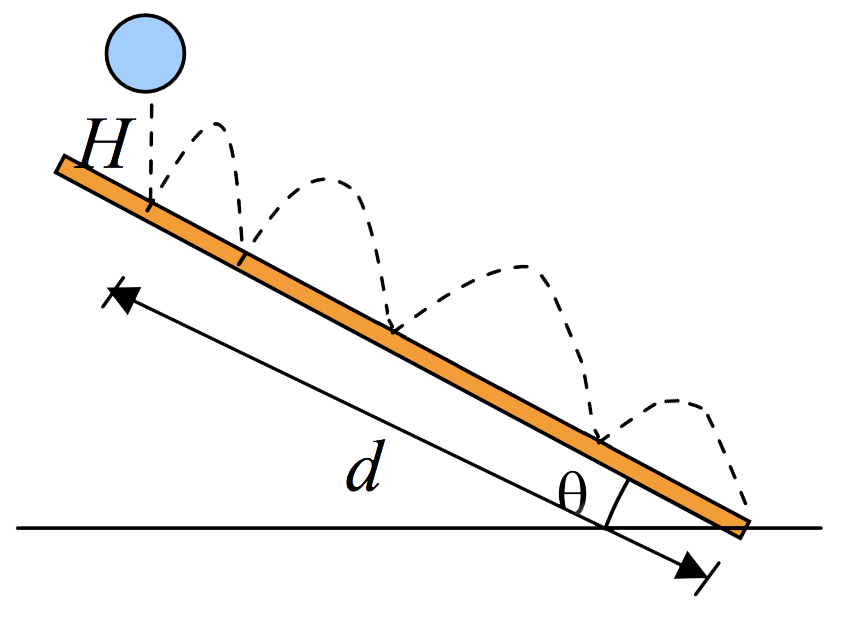
\includegraphics[width=\textwidth,left]{bounce2.png}
\end{minipage}
\end{tabular}

\end{enumerate}

\end{document}
